\chapter{Strutture succinte}



\section{Tipi di dati astratti}
I tipi di dati astratti (ADT, \textit{abstract data type}) sono tipi di dati descritti dal loro comportamento, ossia dalla loro interfaccia e la sua specificazione.
Ad esempio, l'ADT \texttt{stack<T>} è dotato delle seguenti operazioni, chiamate \emph{primitive}:
\begin{verbatim}
  bool     isEmpty()
  T        top()
  stack<T> pop()
  stack<T> push(T)
\end{verbatim}
L'effettivo comportamento delle primitive può essere specificato in diversi modi, ad esempio esplicitandone analiticamente le proprietà:
\begin{gather*}
	\forall S\quad \texttt{s.push(x).top()} = x \\
	\forall S\quad \texttt{s.isEmpty()} \implies \texttt{!S.push(x).pop().isEmpty()}
\end{gather*}
Una volta descritto un ADT è necessario implementarlo, ossia costruire effettivamente una struttura su cui è possibile chiamare le primitive rispettandone la descrizione.
In generale, più implementazioni possono soddisfare le richieste delle primitive: naturalmente, sono particolarmente utili implementazioni che abbiano un basso costo in termini di tempo e spazio.
Ogni ADT ha associato un concetto di \emph{taglia}, che rappresenta genericamente la grandezza di un'istanza: ad esempio, nel caso dello stack la taglia può essere definita come il numero di elementi presenti sulla pila.


\subsection{L'\textit{information theoretical lower bound}}
Per poter caratterizzare le implementazioni degli ADT in base allo spazio che occupano introduciamo alcuni concetti della teoria dell'informazione\footnote{Si veda ad esempio \cite{Cover:06:informtheory} per un approccio moderno a tale campo}.
Il teorema della codifica di sorgente \cite{Shannon:48:theorycommu} (anche noto come primo teorema di Shannon), dà un'informazione fondamentale sullo spazio medio che occupa una struttura dati che può memorizzare $v$ valori:
\begin{theorem}
	\label{thm:shannon}
	Per codificare $v$ valori servono in media $\log_2 v$ bit.
\end{theorem}

Il teorema è ovvio nel caso di rappresentazioni a dimensione fissa.
Per esempio, immaginiamo di dover codificare un'immagine di $100\times100$ pixel in bianco e nero.
Le immagini possibili sono $2^{10000}$, e il teorema afferma che per codificare queste immagini servono in media $10000$ bit.
In effetti, la rappresentazione banale, che rappresenta ogni pixel con un bit, utilizza esattamente $10000$ bit.
Usando meno bit alcune immagini diverse avrebbero, inevitabilmente, la stessa rappresentazione.

Il teorema, però, vale anche per rappresentazioni di dimensione variabile
Ad esempio, si supponga di avere un algoritmo in grado di comprimere tre immagini come le precedenti, ognuna in $100$ bit.
La conseguenza di questo teorema è che esistono altre immagini la cui codifica utilizza più di $10000$ bit, mantenendo la media a $10000$.

Il teorema di Shannon afferma anche che esiste una codifica per rappresentare $v$ valori utilizzando un numero di bit medio in $[\log_2 v,1+\log_2 v)$, assumendo che tutti i $v$ valori siano equiprobabili.

Ci confronteremo spesso con il valore $Z_n:=\log_2 v$, chiamato \emph{information-theoretical lower bound}.
Sulla base di tale valore classifichiamo in base allo spazio le implementazioni di un ADT:
\begin{description}
	\item[struttura implicita] il numero medio di bit occupati è $D_n=Z_n+O(1)$;
	\item[struttura succinta] il numero medio di bit occupati è $D_n=Z_n+o(Z_n)$;
	\item[struttura compatta] il numero medio di bit occupati è $D_n=O(Z_n)$.
\end{description}

È da tenere in considerazione, comunque, che spesso sussiste un tradeoff tra lo spazio occupato da una codifica compressa e la velocità in cui è possibile effettuare operazioni su di essa.
Ad esempio, difficilmente è possibile effettuare operazioni su un file compresso con un algoritmo di compressione general-purpose come \textit{tz2}.



\section{Strutture di rango e selezione}
Le strutture di rango e selezione sono ADT che consistono in un vettore $b$ di lunghezza $n$ su cui è possibile effettuare le primitive $\rank$ e $\select$:
\begin{align*}
	 & \bullet\quad \forall p\leq n\quad \rank_b(p) := \card{\set{i\mid i<p\land b_i=1}} = \sum_{i=0}^n b_i \\
	 & \bullet\quad \forall k\leq \rank_b(n)\quad \select_b(k) := \max\set{p\mid \rank_b(p)\leq k}
\end{align*}

Per esempio, se $b = [0 1 1 0 1 0 1]$ le tabelle di rank e select di $b$ sono descritte in \cref{table:rank_sel}.
\begin{table}[ht]
	\centering
	\begin{subtable}{0.45\textwidth}
		\centering
		\begin{tabular}{c|c}
			$p$ & $\rank_b(p)$ \\ \hline
			0   & 0            \\
			1   & 0            \\
			2   & 1            \\
			3   & 2            \\
			4   & 2            \\
			5   & 3            \\
			6   & 3            \\
			7   & 4
		\end{tabular}
		\caption{$\rank_b(p)$}
	\end{subtable}
	\begin{subtable}{0.45\textwidth}
		\centering
		\begin{tabular}{c|c}
			$k$ & $\select_b(p)$ \\ \hline
			0   & 1              \\
			1   & 2              \\
			2   & 4              \\
			3   & 6              \\
			4   & 7
		\end{tabular}
		\caption{$\select_b(p)$}
	\end{subtable}
	\caption{Operazioni di rango e selezione su $b$.}
	\label{table:rank_sel}
\end{table}

Valgono due proprietà fondamentali per le operazioni di rango e selezione:
\begin{gather*}
	\forall k\quad \rank_b(\select_b(k)) = k \\
	\forall p\quad \select_b(\rank_b(p)) \geq p
\end{gather*}
% TODO: elaborare
Grazie a queste proprietà è possibile ricostruire i valori di $b$ dalle sole query delle operazioni di rango e selezione su di esso.


% TODO: bisognerebbe indagare cosa succede quando la divisione in blocchi e superblocchi non è precisa (e nel caso aggiungere ceiling/floor opportuni)
\subsection{La struttura di Jacobson per il rango}
La struttura di Jacobson fornisce un'implementazione efficiente dell'operazione rango pur consistendo in una rappresentazione succinta dell'array di bit.
La struttura fa uso del cosiddetto "trucco dei quattro russi" \cite{Arlazarov:70:fourrussians}.

Il vettore $b$ di $n$ bit viene diviso in parti uguali, chiamate \emph{superblocchi}, di lunghezza $\log_2^2 n$.
Ogni superblocco viene diviso a sua volta in parti più piccole, dette blocchi, di lunghezza $\frac{1}{2}\log_2 n$, come rappresentato in \cref{fig:jrank}.

% TODO: rifare figura
\begin{figure}[ht]
	\centering
	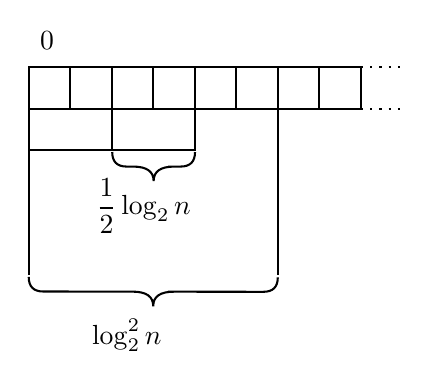
\begin{tikzpicture}[x=0.75pt,y=0.75pt,yscale=-1,xscale=1]
	\draw (150,231) .. controls (149.99,235.67) and (152.32,238) .. (156.99,238.01) -- (199.99,238.07) .. controls (206.66,238.08) and (209.99,240.41) .. (209.98,245.08) .. controls (209.99,240.41) and (213.32,238.09) .. (219.99,238.1)(216.99,238.09) -- (262.99,238.16) .. controls (267.66,238.17) and (269.99,235.84) .. (270,231.17);
	\draw (150,150) -- (150,230);
	\draw (270,150) -- (270,230);
	\draw (150,130) -- (170,130) -- (170,150) -- (150,150) -- cycle;
	\draw (170,130) -- (190,130) -- (190,150) -- (170,150) -- cycle;
	\draw (190,130) -- (210,130) -- (210,150) -- (190,150) -- cycle;
	\draw (210,130) -- (230,130) -- (230,150) -- (210,150) -- cycle;
	\draw (230,130) -- (250,130) -- (250,150) -- (230,150) -- cycle;
	\draw (250,130) -- (270,130) -- (270,150) -- (250,150) -- cycle;
	\draw (270,130) -- (290,130) -- (290,150) -- (270,150) -- cycle;
	\draw (290,130) -- (310,130) -- (310,150) -- (290,150) -- cycle;
	\draw (150,150) -- (190,150) -- (190,170) -- (150,170) -- cycle;
	\draw (190,150) -- (230,150) -- (230,170) -- (190,170) -- cycle;
	\draw (190.22,170.82) .. controls (190.22,175.49) and (192.55,177.82) .. (197.22,177.82) -- (200.17,177.82) .. controls (206.84,177.82) and (210.17,180.15) .. (210.17,184.82) .. controls (210.17,180.15) and (213.5,177.82) .. (220.17,177.82)(217.17,177.82) -- (223.11,177.82) .. controls (227.78,177.82) and (230.11,175.49) .. (230.11,170.82);
	\draw [dash pattern={on 0.84pt off 2.51pt}]  (310,130) -- (330,130);
	\draw [dash pattern={on 0.84pt off 2.51pt}]  (310,150) -- (330,150);

	\draw (179,250) node [anchor=north west][inner sep=0.75pt] [align=left] {$\displaystyle \log_2^2 n$};
	\draw (181,182) node [anchor=north west][inner sep=0.75pt] [align=left] {$\displaystyle \frac{1}{2} \log_2 n$};
	\draw (154,111.4) node [anchor=north west][inner sep=0.75pt] {$0$};
\end{tikzpicture}

	\caption{Divisione di $b$ in superblocchi e blocchi.}
	\label{fig:jrank}
\end{figure}

Si costruiscono quindi due vettori, $S$ e $B$. Per ogni superblocco $i$, $S_i$ contiene il rango del primo elemento di $b$ nel superblocco $i$. Per ogni blocco $j$, $B_j$ contiene la differenza tra il rango del primo elemento del blocco $j$ e il rango del primo elemento del relativo superblocco. Il rango di un elemento $p$ appartenente al superblocco $i$ e al blocco $j$ è quindi uguale a $S_i+B_j$ più il numero di bit a $1$ dall'inizio del blocco $j$ al bit $p$, ossia il rango di $p$ all'interno del sottovettore che coincide con il blocco $j$.

\begin{table}
	\centering
	\begin{tabular}{|c|c|c|c|c|c|c|}
		\hline
		\multirow{2}{*}{$0000$} & $p$        & $0$ & $1$ & $2$ & $3$ & $4$ \\ \cline{2-7}
		                        & $\rank(p)$ & $0$ & $0$ & $0$ & $0$ & $0$ \\ \hline
		\multirow{2}{*}{$0001$} & $p$        & $0$ & $1$ & $2$ & $3$ & $4$ \\ \cline{2-7}
		                        & $\rank(p)$ & $0$ & $0$ & $0$ & $0$ & $1$ \\ \hline
		$\cdots$                &            &     &     &     &     &     \\ \hline
		\multirow{2}{*}{$1111$} & $p$        & $0$ & $1$ & $2$ & $3$ & $4$ \\ \cline{2-7}
		                        & $\rank(p)$ & $0$ & $1$ & $2$ & $3$ & $4$ \\ \hline
	\end{tabular}
	\caption{Rango di ogni possibile blocco di lunghezza $4$.}
	\label{table:example_rank_block4}
\end{table}

I ranghi delle posizioni in un blocco sono salvati in un'apposita tabella, per evitare di doverli calcolare ogni volta. È quindi necessaria una tabella (simile a quanto mostrato in \cref{table:example_rank_block4}) che contiene il rango di ogni posizione, per ogni possibile tipo di blocco. I tipi di blocco possibili sono, in numero:
\begin{equation*}
	2^{\frac{1}{2}\log_2 n} = \left(2^{\log_2 n}\right)^{\frac{1}{2}} = \sqrt{n}
\end{equation*}

Il costo in bit di ogni tabella è
\begin{equation*}
	\underbrace{\frac{1}{2}\log_2 n}_\text{numero di elementi}\cdot \underbrace{\log_2\left(\frac{1}{2}\log_2 n\right)}_\text{costo dei valori di rango}
\end{equation*}
per un totale, per tutte le tabelle, di
\begin{equation*}
	\sqrt n\cdot\frac{1}{2}\log_2 n\cdot \log_2\left(\frac{1}{2}\log_2 n\right)
	\leq \sqrt n\cdot \frac{1}{2}\log_2 n\cdot \log_2(\log_2 n) = o(n) \text{ bit.}
\end{equation*}

Lo spazio occupato dal vettore $S$ è
\begin{equation*}
	\underbrace{\frac{n}{\log_2^2 n}}_\text{numero di superblocchi}\cdot\underbrace{\log_2 n}_\text{costo del singolo valore} = \frac{n}{\log_2 n} = o(n) \text{ bit}
\end{equation*}
Mentre quello occupato dal vettore $B$ è
\begin{equation*}
	\underbrace{\frac{n}{\frac{1}{2}\log_2 n}}_\text{numero di blocchi} \cdot\log_2(\log_2^2 n) =
	\frac{2n}{\log_2 n} 2 \log_2(\log_2 n) = o(n) \text{ bit}
\end{equation*}

% TODO migliorare figura (blocchi di 2 non sono molto rappresentativi)
\begin{figure}
	\centering
	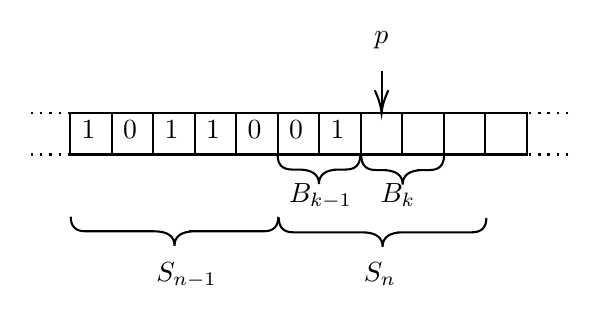
\begin{tikzpicture}[x=0.75pt,y=0.75pt,yscale=-1,xscale=1]
	\draw (100,100) -- (320,100) -- (320,120) -- (100,120) -- cycle;
	\draw (120,100) -- (120,120);
	\draw (140,100) -- (140,120);
	\draw (160,100) -- (160,120);
	\draw (180,100) -- (180,120);
	\draw (200,100) -- (200,120);
	\draw (220,100) -- (220,120);
	\draw (240,100) -- (240,120);
	\draw (260,100) -- (260,120);
	\draw (280,100) -- (280,120);
	\draw (300,100) -- (300,120);
	\draw (250,80) -- (250,98);
	\draw [shift={(250,100)}, rotate = 270] [color={rgb, 255:red, 0; green, 0; blue, 0 }  ][line width=0.75]    (10.93,-3.29) .. controls (6.95,-1.4) and (3.31,-0.3) .. (0,0) .. controls (3.31,0.3) and (6.95,1.4) .. (10.93,3.29);
	\draw (100.25,150) .. controls (100.25,154.67) and (102.58,157) .. (107.25,157) -- (140.25,157) .. controls (146.92,157) and (150.25,159.33) .. (150.25,164) .. controls (150.25,159.33) and (153.58,157) .. (160.25,157)(157.25,157) -- (193.25,157) .. controls (197.92,157) and (200.25,154.67) .. (200.25,150);
	\draw (200.5,150.5) .. controls (200.5,155.17) and (202.83,157.5) .. (207.5,157.5) -- (240.5,157.5) .. controls (247.17,157.5) and (250.5,159.83) .. (250.5,164.5) .. controls (250.5,159.83) and (253.83,157.5) .. (260.5,157.5)(257.5,157.5) -- (293.5,157.5) .. controls (298.17,157.5) and (300.5,155.17) .. (300.5,150.5);
	\draw [dash pattern={on 0.84pt off 2.51pt}] (100,100) -- (80,100);
	\draw [dash pattern={on 0.84pt off 2.51pt}] (100,120) -- (80,120);
	\draw [dash pattern={on 0.84pt off 2.51pt}] (340,120) -- (320,120);
	\draw [dash pattern={on 0.84pt off 2.51pt}] (340,100) -- (320,100);
	\draw (240.25,120.5) .. controls (240.25,125.17) and (242.58,127.5) .. (247.25,127.5) -- (250.17,127.5) .. controls (256.84,127.5) and (260.17,129.83) .. (260.17,134.5) .. controls (260.17,129.83) and (263.5,127.5) .. (270.17,127.5)(267.17,127.5) -- (273.08,127.5) .. controls (277.75,127.5) and (280.08,125.17) .. (280.08,120.5);
	\draw (199.92,120.25) .. controls (199.92,124.92) and (202.25,127.25) .. (206.92,127.25) -- (209.83,127.25) .. controls (216.5,127.25) and (219.83,129.58) .. (219.83,134.25) .. controls (219.83,129.58) and (223.16,127.25) .. (229.83,127.25)(226.83,127.25) -- (232.75,127.25) .. controls (237.42,127.25) and (239.75,124.92) .. (239.75,120.25);
	\draw (245,59.4) node [anchor=north west][inner sep=0.75pt] {$p$};
	\draw (104,102.4) node [anchor=north west][inner sep=0.75pt] {$1$};
	\draw (124,102.4) node [anchor=north west][inner sep=0.75pt] {$0$};
	\draw (144,102.4) node [anchor=north west][inner sep=0.75pt] {$1$};
	\draw (224,102.4) node [anchor=north west][inner sep=0.75pt] {$1$};
	\draw (164,102.4) node [anchor=north west][inner sep=0.75pt] {$1$};
	\draw (204,102.4) node [anchor=north west][inner sep=0.75pt] {$0$};
	\draw (240,170.4) node [anchor=north west][inner sep=0.75pt] {$S_{n}$};
	\draw (140,170.4) node [anchor=north west][inner sep=0.75pt] {$S_{n-1}$};
	\draw (248,132.4) node [anchor=north west][inner sep=0.75pt] {$B_{k}$};
	\draw (204,132.4) node [anchor=north west][inner sep=0.75pt] {$B_{k-1}$};
	\draw (184,102.4) node [anchor=north west][inner sep=0.75pt] {$0$};
\end{tikzpicture}

	\caption{Calcolo di $\rank(p)$.}
	\label{fig:example_rank_p}
\end{figure}

Un'implementazione della struttura succinta di Jacobson per il rango impiega un tempo costante per calcolare il rango di una posizione $p$, dovendo effettuare un accesso ai vettori $S$ e $B$ e uno alla tabella dei tipi di blocco. In effetti l'identificazione del tipo di blocco, stando al criterio di costo della macchina di Turing, è logaritmica in $n$, dovendo scansionare linearmente il blocco che contiene la posizione interessata. Tuttavia, adottando un criterio di costo simile alle macchine reali, questa scansione avviene in tempo costante, poiché un blocco è solitamente contenuto in una o due parole di memoria, recuperate in tempo costante.


% TODO: manca del tutto la revisione di questa subsection
\subsection{Struttura di Clarke per la selezione}
La struttura di Clarke per la selezione è succinta teoricamente, ma in pratica
è raramente utilizzata come descritta perché la sua implementazione è molto
complessa.
L'obiettivo è, dato un vettore $\mathbf{b}$ di valori binari fissato, calcolare
la funzione di selezione
$$
	\mathbf{select_b}(k) = \text{ posizione del } k-\text{esimo } 1
$$
La struttura di Clarke utilizza dei \textit{livelli}, simili a quelli utilizzati
dalla struttura di Jacobson.

\subsubsection{Primo livello}
Il primo livello della struttura di Clarke è un insieme
di valori che rappresentano le posizioni degli $1$ di ordinalità multipla di
$\log_2(n) \cdot \log_2(\log_2(n))$, ossia
$$
	P_i =  \mathbf{select_b}(i \cdot \log_2(n) \cdot \log_2(\log_2(n)))
$$
ossia la posizione del $(i \cdot \log_2(n) \cdot \log_2(\log_2(n)))$-esimo $1$.

\paragraph{Memoria}
La grandezza di questa famiglia, ossia il numero di $P_i$, dipende dal
numero di $i$ che ci sono in $\mathbf{b}$, ma nel caso peggiore, il vettore
è composto unicamente da $1$ e vi saranno $\frac{n}{\log_2(n) \cdot \log_2(\log_2(n))}$ membri.
Ad ognuno di essi va associato un elemento, il quale richiede $\log_2(n)$ bit;
in totale, questo livello occupa
$$
	\frac{n}{\log_2(n) \cdot \log_2(\log_2(n))} \cdot \log_2(n) = o(n) \text{ bit}
$$

\subsubsection{Secondo livello}
Per le posizioni che non sono multiple di $\log_2(n) \cdot \log_2(\log_2(n))$ si utilizza
un secondo livello, che è costruito differentemente in base ad un indice calcolato
per ogni $P_i$:

$$
	\forall i ~ r_i = P_{i + 1} - P_i
$$
che rappresenta la distanza fra l'$(i \cdot \log_2(n) \cdot \log_2(\log_2(n)))$-esimo $1$
e il $((i+1) \cdot \log_2(n) \cdot \log_2(\log_2(n)))$-esimo. Questo
valore, $r_i$, sarà esattamente uguale a $\log_2(n) \cdot \log_2(\log_2(n))$ se e solo se
tra $P_{i}$ e $P_{i+1}$ ci sono unicamente $1$, e sarà maggiore se invece le
due posizioni sono più lontane.
% @TODO: serve un esempio, non si capisce bene. 
I due casi che si considerano dipendono dal valore di $r_i$.

\paragraph{Caso sparso}
Se $r_i \geq (\log_2(n) \cdot \log_2(\log_2(n)))^2$, significa che in $\mathbf{b}$ ci
sono molti $0$ tra gli $1$ contenuti nelle posizioni tra $P_{i}$ e $P_{i+1}$; in questo caso
definiamo $S_i$ come la lista esplicita delle posizioni di tutti gli $1$
in $\mathbf{b}$ tra le due posizioni rappresentate come differenza tra $P_i$.

In questo caso, gli $S_i$ costruiti sono esattamente $\log_2(n)\cdot \log_2(\log_2(n))$,
in quanto stiamo contando gli $1$ in $\mathbf{b}$ tra il $(i \cdot \log_2(n) \cdot \log_2(\log_2(n))$-esimo
$1$ e il $((i+1) \cdot \log_2(n) \cdot \log_2(\log_2(n))$-esimo $1$, e ad ognuno
di essi si associa un numero che in grandezza è minore o uguale a
$\log_2(r_i)$, concludendo che per memorizzare un $S_i$ sono necessari
\begin{align*}
	\log_2(n)\cdot \log_2(\log_2(n)) \cdot \log_2(r_i) & = \frac{(\log_2(n)\cdot \log_2(\log_2(n)))^2}{\log_2(n)\cdot \log_2(\log_2(n))} \cdot \log_2(r_i) \\
	                                                   & \leq \frac{r_i}{\log_2(n)\cdot \log_2(\log_2(n))} \cdot \log_2(r_i)                               \\
	                                                   & \leq \frac{r_i}{\log_2(n)\cdot \log_2(\log_2(n))} \cdot \log_2(n)                                 \\
	                                                   & \leq \frac{r_i}{\log_2(\log_2(n))}                                                                \\
	                                                   & \leq \frac{n}{\log_2(\log_2(n))}   = o(n) \text{ bit}
\end{align*}

\paragraph{Caso denso}
Se $r_i \le (\log_2(n) \cdot \log_2(\log_2(n)))^2$, si memorizzano gli $1$
multipli di $\log_2(r_i)\log_2(\log_2(n))$, ossia partendo dalla posizione $P_i$ si salvano le
posizioni degli $j \cdot \log_2(r_i)\log_2(\log_2(n))$-esimi $1$ come differenze da $P_i$, ossia
$$
	S^i_j = \mathbf{select_b}(j \cdot \log_2(r_i)\log_2(\log_2(n))) - P_i
$$

In questo caso, gli $1$ memorizzati sono $\frac{\log_2(n)\cdot \log_2(\log_2(n))}{\log_2(r_i)\cdot \log_2(\log_2(n))}$.
Ad ognuno di questi si associa un valore in grandezza $\log_2(r_i)$, quindi lo spazio utilizzato
per memorizzare tutti i valori $S^i_j$ sono
$$
	\frac{\log_2(n)\cdot \log_2(\log_2(n))}{\log_2(r_i)\cdot \log_2(\log_2(n))} \log_2(r_i) =
	\frac{\log_2(n)\cdot \log_2(\log_2(n))}{\log_2(\log_2(n))} \leq \frac{r_i}{\log_2(\log_2(n))}
	\leq \frac{n}{\log_2(\log_2(n))} = o(n) \text{ bit}
$$


\subsubsection{Terzo livello}
Se nel secondo livello ci si trova nel caso denso, si utilizza un terzo livello.
Questo livello viene utilizzato esclusivamente per gli $1$ le cui posizioni non sono state
salvate nel secondo livello nel caso denso; pertanto, l'assunto è che
$$
	r_i < (\log_2(n) \log_2(\log_2(n)))^2
$$
Per ognuna di queste posizioni calcoliamo la differenza tra $S^i_j$:
$$
	\forall j ~~ \bar{r}^i_j = S^i_{j+1} - S^i_j
$$
Come nel caso precedente, abbiamo due possibilità in base al valore di $\bar{r}^i_j$, il quale
gode comunque della proprietà
$$
	\forall i, j ~~  \bar{r}^i_j \geq \log_2(r_i) \log_2(\log_2(n))
$$
\paragraph{Caso sparso}
Nel caso in cui $\bar{r}^i_j \geq \log_2(\bar{r}^i_j) \log_2(r_i) \log_2(\log_2(n))^2$,
si memorizzano esplicitamente tutte le posizioni degli $1$ tra $S^i_j$ e $S^i_{j+1}$
con dei valori $T^i_{j,k}$ come differenze tra $S^i_j$. In questo caso,
il consumo di memoria è
$$
	(\log_2(r_i)\cdot \log_2(\log_2(n)) \cdot \log_2(\bar{r}^i_j) \leq
	\frac{\log_2(r_i) \cdot \log_2(\log_2(n))^2 \log_2(\bar{r}^i_j)}{\log_2(\log_2(n))}
	\leq \frac{\bar{r}^i_j}{\log_2(\log_2(n))} = o(n) \text{ bit}
$$
\paragraph{Caso denso}
Nel caso in cui $\bar{r}^i_j \le \log_2(\bar{r}^i_j) \log_2(r_i) \log_2(\log_2(n))^2$,
significa che ci sono pochi $0$ tra $S^i_j$ e $S^i_{j+1}$ e
si utilizza il four-russians trick. Inizialmente osserviamo quanto segue.
\begin{oss}
	\begin{align*}
		\log_2(\bar{r}^i_j) \leq \log_2(r_i) & \leq \log_2(\log_2(n)\cdot \log_2(\log_2(n)))^2     \\
		                                     & = 2 \log_2(\log_2(n)) + 2 \log_2(\log_2(\log_2(n))) \\
		                                     & \leq 4 \log_2(\log_2(n))
	\end{align*}
\end{oss}
\begin{oss}
	$$
		\bar{r}^i_j < \log_2(\bar{r}^i_j) \cdot \log_2(r_i) \cdot (\log_2(\log_2(n))^2
		\leq 16(\log_2\log_2(n))^4
	$$
\end{oss}
Lo spazio necessario per utilizzare il four-russians trick è quanto segue.
Servono $2^{\bar{r}^i_j}$ enumerazioni di `sottovettori',
ossia la dimensione tra $S^i_j$ e $S^i_{j+1}$,
che è la parte che va memorizzata esplicitamente; per ognuna di queste
enumerazioni è necessario salvare la posizione di $\bar{r}^i_j$ $1$ utilizzando
memoria al massimo $\log_2(\bar{r}^i_j)$:
\begin{align*}
	2^{\bar{r}^i_j} \cdot \bar{r}^i_j \cdot \log_2(\bar{r}^i_j) & \leq
	2^{16(\log_2\log_2(n))^4} \cdot 16(\log_2\log_2(n))^4 \cdot \log_2(16(\log_2\log_2(n))^4)                                  \\
	                                                            & = 16(\log_2\log_2(n))^8 \log_2(16(\log_2\log_2(n))^4) = o(n)
\end{align*}


\subsubsection{Complessità totale in spazio}
In totale, per memorizzare $\mathbf{b}$ e i possibili tre livelli di struttura,
sono necessari $o(n)$ bit per il primo livello e, in base a come è fatto il secondo livello
$$
	\sum^{\frac{n}{\log_2(n)\cdot \log_2(\log_2(n))}} \frac{P_{i+1} - P_i}{\log_2(\log_2(n)}
	= \frac{P_n - P_0}{\log_2(\log_2(n))}
	\leq \frac{n}{\log_2(\log_2(n))} = o(n) \text{ bit}
$$
più $o(n)$ bit per il terzo livello. Quindi, la struttura di Clarke occupa
spazio $n + o(n)$ e ha tempo di accesso costante, pertanto è
una struttura \textbf{succinta}.

\begin{figure}
	\centering
	\tikzset{every picture/.style={line width=0.75pt}} %set default line width to 0.75pt        

	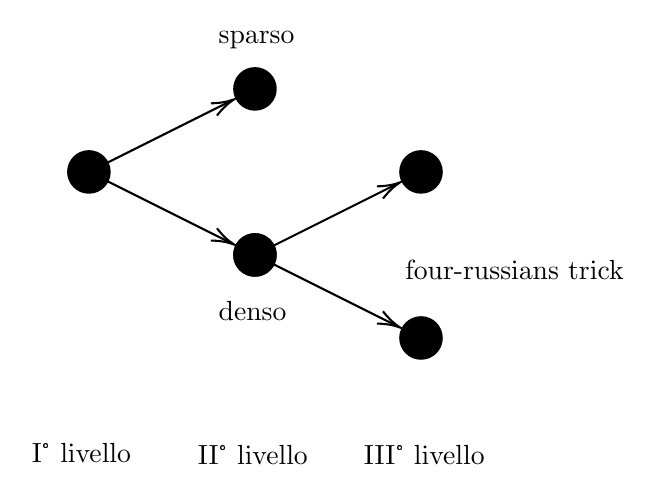
\begin{tikzpicture}[x=0.75pt,y=0.75pt,yscale=-1,xscale=1]
		%uncomment if require: \path (0,300); %set diagram left start at 0, and has height of 300

		%Shape: Circle [id:dp9914836432536758] 
		\draw  [fill={rgb, 255:red, 0; green, 0; blue, 0 }  ,fill opacity=1 ] (70,101) .. controls (70,95.48) and (74.48,91) .. (80,91) .. controls (85.52,91) and (90,95.48) .. (90,101) .. controls (90,106.52) and (85.52,111) .. (80,111) .. controls (74.48,111) and (70,106.52) .. (70,101) -- cycle ;
		%Shape: Circle [id:dp09703813871749656] 
		\draw  [fill={rgb, 255:red, 0; green, 0; blue, 0 }  ,fill opacity=1 ] (150,61) .. controls (150,55.48) and (154.48,51) .. (160,51) .. controls (165.52,51) and (170,55.48) .. (170,61) .. controls (170,66.52) and (165.52,71) .. (160,71) .. controls (154.48,71) and (150,66.52) .. (150,61) -- cycle ;
		%Straight Lines [id:da8346853138498954] 
		\draw    (80,101) -- (148.21,66.89) ;
		\draw [shift={(150,66)}, rotate = 153.43] [color={rgb, 255:red, 0; green, 0; blue, 0 }  ][line width=0.75]    (10.93,-3.29) .. controls (6.95,-1.4) and (3.31,-0.3) .. (0,0) .. controls (3.31,0.3) and (6.95,1.4) .. (10.93,3.29)   ;
		%Shape: Circle [id:dp4565729376211175] 
		\draw  [fill={rgb, 255:red, 0; green, 0; blue, 0 }  ,fill opacity=1 ] (150,141) .. controls (150,146.52) and (154.48,151) .. (160,151) .. controls (165.52,151) and (170,146.52) .. (170,141) .. controls (170,135.48) and (165.52,131) .. (160,131) .. controls (154.48,131) and (150,135.48) .. (150,141) -- cycle ;
		%Straight Lines [id:da8127484960209145] 
		\draw    (80,101) -- (148.21,135.11) ;
		\draw [shift={(150,136)}, rotate = 206.57] [color={rgb, 255:red, 0; green, 0; blue, 0 }  ][line width=0.75]    (10.93,-3.29) .. controls (6.95,-1.4) and (3.31,-0.3) .. (0,0) .. controls (3.31,0.3) and (6.95,1.4) .. (10.93,3.29)   ;
		%Shape: Circle [id:dp546530222511162] 
		\draw  [fill={rgb, 255:red, 0; green, 0; blue, 0 }  ,fill opacity=1 ] (150,141) .. controls (150,135.48) and (154.48,131) .. (160,131) .. controls (165.52,131) and (170,135.48) .. (170,141) .. controls (170,146.52) and (165.52,151) .. (160,151) .. controls (154.48,151) and (150,146.52) .. (150,141) -- cycle ;
		%Shape: Circle [id:dp1691093585413369] 
		\draw  [fill={rgb, 255:red, 0; green, 0; blue, 0 }  ,fill opacity=1 ] (230,101) .. controls (230,95.48) and (234.48,91) .. (240,91) .. controls (245.52,91) and (250,95.48) .. (250,101) .. controls (250,106.52) and (245.52,111) .. (240,111) .. controls (234.48,111) and (230,106.52) .. (230,101) -- cycle ;
		%Straight Lines [id:da17118221437478087] 
		\draw    (160,141) -- (228.21,106.89) ;
		\draw [shift={(230,106)}, rotate = 153.43] [color={rgb, 255:red, 0; green, 0; blue, 0 }  ][line width=0.75]    (10.93,-3.29) .. controls (6.95,-1.4) and (3.31,-0.3) .. (0,0) .. controls (3.31,0.3) and (6.95,1.4) .. (10.93,3.29)   ;
		%Shape: Circle [id:dp8870903616648642] 
		\draw  [fill={rgb, 255:red, 0; green, 0; blue, 0 }  ,fill opacity=1 ] (230,181) .. controls (230,186.52) and (234.48,191) .. (240,191) .. controls (245.52,191) and (250,186.52) .. (250,181) .. controls (250,175.48) and (245.52,171) .. (240,171) .. controls (234.48,171) and (230,175.48) .. (230,181) -- cycle ;
		%Straight Lines [id:da2110125336208042] 
		\draw    (160,141) -- (228.21,175.11) ;
		\draw [shift={(230,176)}, rotate = 206.57] [color={rgb, 255:red, 0; green, 0; blue, 0 }  ][line width=0.75]    (10.93,-3.29) .. controls (6.95,-1.4) and (3.31,-0.3) .. (0,0) .. controls (3.31,0.3) and (6.95,1.4) .. (10.93,3.29)   ;

		% Text Node
		\draw (51,230) node [anchor=north west][inner sep=0.75pt]   [align=left] {I° livello};
		% Text Node
		\draw (131,231) node [anchor=north west][inner sep=0.75pt]   [align=left] {II° livello};
		% Text Node
		\draw (211,231) node [anchor=north west][inner sep=0.75pt]   [align=left] {III° livello};
		% Text Node
		\draw (141,162) node [anchor=north west][inner sep=0.75pt]   [align=left] {denso};
		% Text Node
		\draw (141,32) node [anchor=north west][inner sep=0.75pt]   [align=left] {sparso};
		% Text Node
		\draw (231,142) node [anchor=north west][inner sep=0.75pt]   [align=left] {four-russians trick};
	\end{tikzpicture}
	\caption{Struttura di Clarke per la selezione.}
\end{figure}



\section{Alberi binari}
Un albero è un grafo non orientato, connesso e aciclico.
Un albero con radice è un albero in cui si elegge un vertice radice. I vertici adiacenti alla radice sono i suoi figli, che danno origine a sottoalberi. I vertici che danno origine a sottoalberi composti unicamente dalla radice sono detti foglie, o nodi esterni. I rimanenti nodi in un albero sono detti nodi interni.
Un albero binario è un albero radicato in cui ogni nodo interno ha due figli.
Equivalentemente si possono definire gli alberi binari induttivamente: un albero binario è una foglia $\emptyset$, oppure, se $L$ e $R$ sono alberi binari, è una coppia $(L,R)$ composta da una radice a cui sono connessi i sottoalberi $L$ e $R$.

% TODO: migliorare figura del passo induttivo: la radice dovrebbe essere adiacente alle radici dei sottoalberi
\begin{figure}
	\begin{subfigure}{0.45\textwidth}
	\begin{center}
		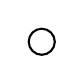
\begin{tikzpicture}
			\node [circle,draw]{};
		\end{tikzpicture}
	\end{center}
	\caption{Foglia}
\end{subfigure}
\begin{subfigure}{0.45\textwidth}
	\begin{center}
		\begin{tikzpicture}[subtree/.style={isosceles triangle,draw,shape border rotate=90}]
			\node[circle,draw] {}
			child { node[subtree] {$T_1$} }
			child { node[subtree] {$T_2$} };
		\end{tikzpicture}
	\end{center}
	\caption{Radice con due sottoalberi}
\end{subfigure}

	\caption{Definizione induttiva di albero binario.}
	\label{fig:btree_inductive}
\end{figure}

Un albero può essere \emph{ancillare}, cioè organizzare dati contenuti nei nodi interni o nelle foglie (tipicamente esclusivamente una delle due opzioni). Le strutture costruite per alberi privi di dati possono tipicamente essere generalizzate al caso di alberi ancillari.

Dato un albero binario, chiameremo $E$ l'insieme dei nodi esterni (foglie), $I$ l'insieme dei nodi interni e $n:=\card{I}$.
Definiamo inoltre le funzioni $\trext$ e $\trint$, definite rispettivamente come il numero di foglie e nodi interni di un dato albero binario.

\begin{theorem}\label{thm:btree_leaves}
	In un albero binario, il numero di foglie è uguale al numero di nodi interni più uno:
	\begin{equation*}
		\card E = \card I + 1
	\end{equation*}
\end{theorem}
\begin{proof}
	Effettuando induzione strutturale sulla definizione di albero binario:
	\begin{itemize}
		\item $\trext(\emptyset)=1$, $\trint(\emptyset)=0$.
		\item siano $L, R$ due alberi binari. Vale
		      \begin{equation*}
			      \trext((L,R)) = \trext(L) + \trext(R) = \trint(L) + 1 + \trint(R) + 1 = \trint((L, R))  + 1
		      \end{equation*}
	\end{itemize}
\end{proof}

\begin{corollario}
	Ogni albero con $n$ nodi interni ha in totale $2n+1$ nodi.
\end{corollario}

\begin{theorem}\label{thm:catalano}
	Il numero di alberi binari con $n$ nodi interni è $C_n$, dove $C_n$ è l'$n$-esimo numero di Catalano:
	\begin{equation*}
		C_n := \frac{1}{n+1}\binom{2n}{n}
	\end{equation*}
\end{theorem}
\begin{corollario}
	$\log_2(C_n)=2n-O(\log n)$.
\end{corollario}
\begin{proof}
	Ricordando l'approssimazione di Stirling per il fattoriale:
	\begin{equation*}
		x! \sim \sqrt{2\pi x} \left(\frac{x}{e}\right)^x
	\end{equation*}
	si ha che
	\begin{align*}
		C_n = \frac{1}{n+1}\binom{2n}{n} & = \frac{1}{n+1}\cdot\frac{(2n)!}{n!(2n-n)!}                                                             \\
		                                 & = \frac{(2n)!}{(n+1)(n!)^2}                                                                             \\
		                                 & \sim \frac{\sqrt{4\pi n}\left(\frac{2n}{e}\right)^{2n}}{(n+1)\cdot 2\pi n\left(\frac{n}{e}\right)^{2n}} \\
		                                 & = \frac{1}{n+1}\cdot \frac{1}{\sqrt{\pi n}}\cdot 2^{2n}                                                 \\
		                                 & \approx \frac{2^{2n}}{\sqrt{\pi n^3}}
	\end{align*}
	da cui
	\begin{align*}
		\log_2(C_n) & \approx \log_2\left(\frac{2^{2n}}{\sqrt{\pi n^3}}\right) \\
		            & = \log_2(2^{2n}) - \log_2(\sqrt{\pi n^3})                \\
		            & = 2n-\frac 12 \log_2(\pi n^3)                          \\
		            & = 2n-O(\log n) \text. \qedhere
	\end{align*}
\end{proof}
\begin{corollario}\label{corol:bitree:itlb}
	L'information theoretical lower bound in bit per gli alberi binari è
	\begin{equation*}
		Z_n = 2n-O(\log n) \text.
	\end{equation*}
\end{corollario}


\subsection{Una struttura succinta per alberi binari}
Per costruire una struttura succinta per gli alberi binari, definiamo tre operazioni fondamentali in cui possono consistere le query alla struttura dati: le operazioni $\trleft$ e $\trright$, che restituiscono rispettivamente il figlio sinistro e destro di un dato nodo, e l'operazione $\trparent$, che restituisce il genitore di un dato nodo.

Per rappresentare un albero binario con $n$ nodi interni $I$, numeriamo i nodi da $0$ a $2n$ seguendo una visita in ampiezza, come rappresentato in \cref{fig:btree_rappr_num}.
Costruiamo quindi un vettore $v$ (\cref{fig:btree_rappr_vec}), di lunghezza $2n+1$ e tale che
\begin{equation*}
	\forall i\in\set{0,\dots,2n},\qquad v_i = \begin{cases}
		1 & \text{se il nodo $i$ appartiene a $I$} \\
		0 & \text{altrimenti}
	\end{cases}
\end{equation*}

\begin{figure}
	\centering
	\begin{subfigure}[t]{0.45\textwidth}
	\centering
	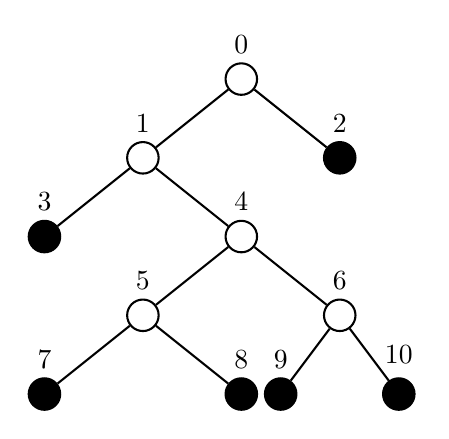
\begin{tikzpicture}[
			every node/.style={circle, draw, minimum size=4mm, inner sep=0.5mm},
			level distance=10mm,
			level 1/.style={sibling distance=25mm},
			level 2/.style={sibling distance=25mm}]
		\node [label=above:{0}]{}
		child {
		node [label=above:{1}] {}
		child {node[fill, label=above:{3}]{}}
		child {
		node[label=above:{4}]{}
		child {
		node [label=above:{5}]{}
		child {node[fill,label=above:{7}]{}}
		child {node[fill,label=above:{8}]{}}
		}
		child {
		node[label=above:{6}]  {}
		[level distance=10mm ,sibling distance=15mm]
		child {node[fill,label=above:{9}] {}}
		child {node[fill,label=above:{10}] {}}
		}
		}
		}
		child {node [fill, label=above:{2}]{}};
	\end{tikzpicture}

	\caption{Albero binario numerato.}
	\label{fig:btree_rappr_num}
\end{subfigure}
\begin{subfigure}[t]{0.45\textwidth}
	\centering
	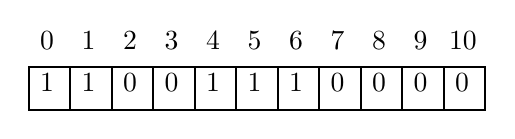
\begin{tikzpicture}[x=0.75pt,y=0.75pt,yscale=-1,xscale=1]
		\draw   (160,120) -- (180,120) -- (180,140.67) -- (160,140.67) -- cycle;
		\draw   (180,120) -- (200,120) -- (200,140.67) -- (180,140.67) -- cycle;
		\draw   (200,120) -- (220,120) -- (220,140.67) -- (200,140.67) -- cycle;
		\draw   (220,120) -- (240,120) -- (240,140.67) -- (220,140.67) -- cycle;
		\draw   (240,120) -- (260,120) -- (260,140.67) -- (240,140.67) -- cycle;
		\draw   (260,120) -- (280,120) -- (280,140.67) -- (260,140.67) -- cycle;
		\draw   (280,120) -- (300,120) -- (300,140.67) -- (280,140.67) -- cycle;
		\draw   (300,120) -- (320,120) -- (320,140.67) -- (300,140.67) -- cycle;
		\draw   (320,120) -- (340,120) -- (340,140.67) -- (320,140.67) -- cycle;
		\draw   (340,120) -- (360,120) -- (360,140.67) -- (340,140.67) -- cycle;
		\draw   (360,120) -- (380,120) -- (380,140.67) -- (360,140.67) -- cycle;
		\draw (164,101.4) node [anchor=north west][inner sep=0.75pt]    {$0$};
		\draw (184,101.4) node [anchor=north west][inner sep=0.75pt]    {$1$};
		\draw (204,101.4) node [anchor=north west][inner sep=0.75pt]    {$2$};
		\draw (224,101.4) node [anchor=north west][inner sep=0.75pt]    {$3$};
		\draw (244,101.4) node [anchor=north west][inner sep=0.75pt]    {$4$};
		\draw (264,101.4) node [anchor=north west][inner sep=0.75pt]    {$5$};
		\draw (284,101.4) node [anchor=north west][inner sep=0.75pt]    {$6$};
		\draw (304,101.4) node [anchor=north west][inner sep=0.75pt]    {$7$};
		\draw (324,101.4) node [anchor=north west][inner sep=0.75pt]    {$8$};
		\draw (344,101.46) node [anchor=north west][inner sep=0.75pt]    {$9$};
		\draw (361,101.4) node [anchor=north west][inner sep=0.75pt]    {$10$};
		\draw (164,121.4) node [anchor=north west][inner sep=0.75pt]    {$1$};
		\draw (184,121.4) node [anchor=north west][inner sep=0.75pt]    {$1$};
		\draw (204,121.4) node [anchor=north west][inner sep=0.75pt]    {$0$};
		\draw (224,121.4) node [anchor=north west][inner sep=0.75pt]    {$0$};
		\draw (244,121.4) node [anchor=north west][inner sep=0.75pt]    {$1$};
		\draw (264,121.4) node [anchor=north west][inner sep=0.75pt]    {$1$};
		\draw (284,121.4) node [anchor=north west][inner sep=0.75pt]    {$1$};
		\draw (304,121.4) node [anchor=north west][inner sep=0.75pt]    {$0$};
		\draw (324,121.4) node [anchor=north west][inner sep=0.75pt]    {$0$};
		\draw (344,121.46) node [anchor=north west][inner sep=0.75pt]    {$0$};
		\draw (364,121.4) node [anchor=north west][inner sep=0.75pt]    {$0$};
	\end{tikzpicture}
	\caption{Vettore associato all'albero.}
	\label{fig:btree_rappr_vec}
\end{subfigure}

	\caption{Un albero binario e il suo vettore associato.}
\end{figure}

Studiamo ora come produrre i risultati delle query di $\trleft$, $\trright$, e $\trparent$ a partire dal vettore $v$.
Si consideri, all'interno di un albero $T$, una terna di nodi $p,q,q+1$, dove $p$ è il genitore e $q$ e $q+1$ i figli.
Sia $T'$ il sottoalbero radicato nella stessa radice di $T$ contenente tutti i nodi di indice minore di $q$, come rappresentato in figura \ref{fig:btree_rappr_step}.
Si tenga presente che alcuni nodi interni nell'albero $T$, in particolare quelli che seguono $p$, diventano foglie in $T'$.
Non esistono quindi in $T'$ nodi interni (ossia bit a $1$ nella rappresentazione binaria) successivi a $p$.

Il numero di nodi interni minori di $p$, ossia il numero di nodi interni in $T'$, è uguale al rango di $p$ in $v$. Applicando il \cref{thm:btree_leaves}, calcoliamo che il numero complessivo di nodi minori di $q$, cioè il numero di nodi dell'albero $T'$, è
\begin{equation}\label{eq:btree:left_child}
	\trleft(p) = q = \trint(T')+\trext(T') = 2\cdot\trint(T')+1 = 2\cdot\rank(p)+1 \text.
\end{equation}
Mentre per il figlio destro vale, ovviamente
\begin{equation}\label{eq:btree:right_child}
	\trright(p) = q+1 = 2\cdot\rank(p)+2 \text.
\end{equation}

\begin{figure}
	\centering
	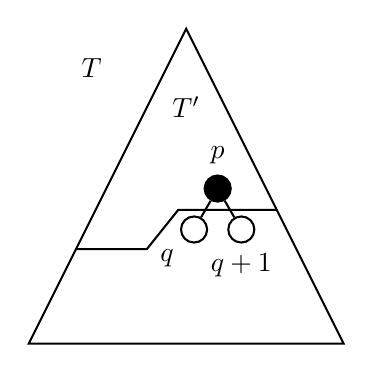
\begin{tikzpicture}[child/.style={draw,circle},father/.style={child,fill}]
  \draw (0,0) -- (4,0) -- (2,4) -- cycle;
  \draw (0.6,1.2) -- (1.5,1.2) -- (1.9,1.7) -- (3.15,1.7);
  \node (p) [father,label=above:{$p$}] at (2.4,1.97) {};
  \node (q) [child,label=below left:{$q$}] at (2.1,1.45) {};
  \node (qp) [child,label=below:{$q+1$}] at (2.7,1.45) {};
  \draw (p) -- (q);
  \draw (p) -- (qp);
  \node at (2,3) {$T'$};
  \node at (0.8,3.5) {$T$};
\end{tikzpicture}

	\caption{Sottoalbero $T'$ di $T$ utilizzato per calcolare $q$ e $q+1$.}
	\label{fig:btree_rappr_step}
\end{figure}

Per implementare l'operazione $\trparent$, si osservi che in virtù delle equazioni (\ref{eq:btree:left_child}) e (\ref{eq:btree:right_child}) vale
\begin{equation*}
	\begin{cases}
		\rank(p)=\dfrac{q}{2}-\dfrac12 & \quad\text{per $q$ dispari} \\[2ex]
		\rank(p)=\dfrac{q}{2}-1        & \quad\text{per $q$ pari}
	\end{cases}
\end{equation*}
da cui si ricava
\begin{equation*}
	\rank(p)=\floor{\frac q2-\frac 12}
\end{equation*}
e quindi, essendo $\select(\rank(p))=p$ poiché $v_p=1$:
\begin{equation*}
	p=\select(\rank(p))=\select\left(\floor{\frac q2-\frac 12}\right) \text.
\end{equation*}

È quindi possibile fare uso di una struttura per rappresentare il vettore $v$ che sia succinta rispetto all'information theoretical lower bound trovato al \cref{corol:bitree:itlb}:
\begin{align*}
	D_n & = 2n+1+o(n)    \\
	Z_n & = 2n-O(\log n)
\end{align*}



\section{Sequenze monotone}
Sia data una sequenza monotona di $n$ numeri naturali
\begin{equation*}
	x_0\leq x_1\leq \dots \leq x_{n-1}
\end{equation*}
Con un valore $u$, chiamato \emph{dimensione dell'universo}, tale che
\begin{equation*}
	\exists u ~ \forall i ~ x_i < u \text.
\end{equation*}

Dato un naturale $i<n$, si vuole ottenere l'elemento di indice $i$ della sequenza.


\subsection{La struttura di Elias-Fano}
Per evitare di usare un vettore di $n\cdot\log_2 u$ bit, viene definito un valore limite $l$:
\begin{equation*}
	l := \max\set{0,\floor{\log_2\left(\frac{u}{n}\right)}}\text.
\end{equation*}
La rappresentazione di Elias-Fano estrae da ogni intero $x_i$ la parte $l_i:=x_i\mod 2^l$, formata dai $l$ bit meno significativi. Per memorizzare le parti $l_i$ si fa uso di un vettore $L$ di $n$ elementi, ciascuno di $l$ bit.

Per le parti più significative, si calcolano i valori $u_i:=\floor{\frac{x_i}{2^l}}-\floor{\frac{x_{i-1}}{2^l}}$ (dove implicitamente $x_{-1}=0$), che vengono memorizzati in codifica unaria in una porzione di memoria $U$.
Nell'analisi prenderemo in considerazione il caso sparso ($u>n$), quindi assumeremo $l=\floor{\log_2\left(\frac{u}{n}\right)}$.


\subsubsection{Costo in spazio}
Il vettore $L$ ha costo, ovviamente, $l\cdot n$ bit.
Il numero di bit richiesti a memorizzare ciascun $u_i$ è uguale a $u_i+1$ ($u_i$ zeri e un $1$). In tutto
\begin{align*}
	\sum_{i=0}^{n-1}(u_i+1) & = \sum_{i=0}^{n-1}\left(\floor{\frac{x_i}{2^l}}-\floor{\frac{x_{i-1}}{2^l}}+1\right) \\
	                        & = n + \floor{\frac{x_{n-1}}{2^l}} \leq n + \frac{u}{2^l}                             \\[1ex]
	                        & = n + \frac{u}{2^{\floor{\log_2\frac{u}{n}}}}
\end{align*}
Se $u/n$ è una potenza di $2$, questo numero è uguale a $2n$, altrimenti è limitato da $3n$:
\begin{align*}
	 & \leq n+\frac{u}{2^{\log_2\frac{u}{n}-1}} \\[1ex]
	 & = n+\frac{2u}{u/n} = 3n \text.
\end{align*}
Considerando entrambe le parti, questa struttura occupa in spazio $l\cdot n$ bit per la parte inferiore e $2n$ o $3n$ bit per la parte superiore.
In totale, quindi, il costo è di $(l+2)n$ o $(l+3)n$ bit.
Ricordando l'ipotesi che $l=\floor{\log_2(u/n)}$, vale
\begin{equation*}
	\lceil \log_2(u/n) \rceil =
	\begin{cases}
		l & u/n \text{ è una potenza di } 2 \\
		l +1                                \\
	\end{cases}
\end{equation*}
Complessivamente, quindi, la struttura occupa un numero di bit di al più
\begin{equation*}
	D_n = 2n+n\ceil{\log_2\frac un} \text.
\end{equation*}


Per ricavare la parte più significativa di $x_i$ è necessario contare il numero di zeri fino all'$1$ di indice $i$ in $U$. Questo numero è uguale a $\select(i)-i$, quindi:
\begin{equation*}
	x_i=(\select(i)-i)2^l+l_i
\end{equation*}

Contando strutture succinte di rango e selezione rendere più efficiente il calcolo degli $x_i$, si ottiene un costo in spazio complessivo di
\begin{equation*}
	D_n = 2n+n\ceil{\log_2\frac un}+o(n) \text.
\end{equation*}


\subsection{Information theoretical lower bound}
Le possibili sequenze monotone di $n$ interi limitati da $u$ corrispondono ai possibili multisottoinsiemi dell'insieme $\set{0,\dots,u-1}$ di cardinalità $n$, nonché alle soluzioni dell'equazione
\begin{equation}\label{eq:seqmon}
	c_0+c_1+\dots+c_{u-1} = n
\end{equation}
dove $c_i$ è il numero di occorrenze dell'intero $i$ nella sequenza.

Per contare le possibili soluzioni si può utilizzare la tecnica \textit{stars and bars}, in
cui si utilizza una stringa costruita utilizzando $n$ stelline e $u-1$ barrette per rappresentare una soluzione all'equazione (\ref{eq:seqmon}). Ad esempio:
\begin{equation*}
	| \starsymb || \starsymb \starsymb || \starsymb | \starsymb
\end{equation*}

Il valore complessivo della sequenza è $n$ e va distribuito in $u$ spazi, delineati dalle $u-1$ barrette.
L'interpretazione della stringa appena mostrata è $ c_0 = 0, c_1 = 1, c_2 = 0, c_3 = 2, c_4 = 0, c_5 = 1, c_6 = 1 $.
Il numero di soluzioni possibili è uguale al numero di stringhe costruite in questo modo, che equivale al numero di modi di scegliere $u-1$ posizioni in cui inserire barre in una stringa di $n+u-1$ simboli, ossia $\binom{n+u-1}{u - 1}$.

% TODO: spiegare calcoli e approssimazioni
Facendo uso dell'approssimazione di Stirling per il coefficiente binomiale\footnote{$\log\binom AB \approx B\log\frac AB+(A-B)\log\frac{A}{A-B}$. In questo caso $A:=u+n-1$ e $B:=n$, quindi per $n\ll u$ il secondo addendo si annulla.}:
\begin{align*}
	Z_n & = \log_2\binom{n+u-1}{u - 1} = \log_2\binom{n+u-1}{n}              \\
	    & \approx n\log_2\frac{u+n-1}{n} =                                   \\
	    & = n\log_2\left(\frac un\left(1+\frac nu - \frac 1u\right)\right) = \\
	    & = n\log_2\frac un + n\log_2\left(1+\frac nu-\frac 1u\right)        \\
	    & \sim n\log_2\frac un + \frac{n^2}{u} \approx n\log_2\frac un
\end{align*}

Quindi la struttura è compatta:
\begin{equation*}
	D_n = 2n+n\ceil{\log_2\frac un}+o(n) = O(Z_n)
\end{equation*}



\section{Parentesi ben bilanciate}
L'insieme $D_k$, con $k\in\N$, contiene le parole di Dyck di semilunghezza $k$, cioè composte da $2k$ parentesi ben bilanciate (di cui $k$ aperte e $k$ chiuse). Gli insiemi $D_k$ sono definiti induttivamente:
\begin{itemize}
	\item $\emptyword\in D_0$
	\item $x\in D_n,y\in D_m\Rightarrow xy\in D_{n+m}$
	\item $x\in D_n\Rightarrow (x)\in D_{n+1}$
\end{itemize}
Equivalentemente
\begin{itemize}
	\item $\emptyword\in D_0$
	\item $x\in D_n,y\in D_m\Rightarrow (x)y\in D_{n+m+1}$
\end{itemize}

Per ogni parola di Dyck viene definita la funzione di eccesso, che rappresenta la profondità, in numero di parentesi innestate, di ogni posizione. Per $i\in\set{0,\dots,\len w}$:
\begin{equation*}
	E_w(i) = \card{\set{j < i \mid w_j = (~ }} - \card{\set{j\leq i \mid w_j =~)~ }}
\end{equation*}
Si noti che la funzione di eccesso non può scendere sotto il valore che ha nella posizione di una parentesi aperta finché non raggiunge la rispettiva chiusa.

\begin{figure}[ht]
	\centering
	\begin{tikzpicture}[point/.style={fill,circle,inner sep=1pt}]
	\draw[->] (-.5,0) -- (8,0)	node[right] {$i$};
	\draw[->] (-.5,0) -- (-.5,3.5)	node[above] {$E(i)$};

	\node (i0) [point,label=above:{$($}] at (0,0) {};
	\node (i1) [point,label=above:{$($}] at (1,1) {};
	\node (i2) [point,label=above:{$)$}] at (2,1) {};
	\node (i3) [point,label=above:{$($}] at (3,1) {};
	\node (i4) [point,label=above:{$($}] at (4,2) {};
	\node (i5) [point,label=above:{$)$}] at (5,2) {};
	\node (i6) [point,label=above:{$)$}] at (6,1) {};
	\node (i7) [point,label=above:{$)$}] at (7,0) {};

	\draw (i0) -- (i1) -- (i2) -- (i3) -- (i4) -- (i5) -- (i6) -- (i7);
\end{tikzpicture}

	\caption{Funzione di eccesso per la parola $(()(()))$.}
	\label{fig:func_excess}
\end{figure}

Le parole di Dyck si classificano sulla base della loro funzione di eccesso in due categorie:
\begin{description}
	\item[fortemente bilanciate] la funzione non ha zeri se non per il primo e l'ultimo simbolo;
	\item[debolmente bilanciate] la funzione ha uno zero in una posizione $i$ diversa dalla prima e dall'ultima. Il prefisso di lunghezza $i+1$ della parola è fortemente bilanciato.
\end{description}

L'ADT che vogliamo descrivere per le stringhe di parentesi ben bilanciate si compone delle seguenti primitive, che hanno come input una posizione $p$:
\begin{description}
	\renewcommand{\dyfindopen}{\mathbf{find\_open}}
	\renewcommand{\dyfindclosed}{\mathbf{find\_closed}}
	\renewcommand{\dyenclose}{\mathbf{enclose}}
	\item[$\dyfindopen$] restituisce la posizione della parentesi aperta corrispondente alla chiusa in posizione $p$. Coincide con la prima posizione $q>p$ in cui la funzione di eccesso è uguale a quella di $p$;
	\item[$\dyfindclosed$] restituisce la posizione della parentesi chiusa corrispondente all'aperta in posizione $p$. Coincide con l'ultima posizione $q<p$ in cui la funzione di eccesso è uguale a quella di $p$;
	\item[$\dyenclose$] restituisce la posizione della parentesi aperta della coppia che racchiude la parentesi in posizione $p$.
\end{description}


\subsection{Una struttura compatta per parentesi ben bilanciate}
Una struttura compatta a tempo logaritmico per le parentesi bilanciate prevede di dividere la parola $w$, di lunghezza $n$, in blocchi di lunghezza $l$, ottenendo $k=\ceil{n/l}$ blocchi (l'ultimo dei quali può avere lunghezza inferiore a $l$).

Sia $p$ la posizione di una parentesi nel blocco $B_i$. La parentesi $w_p$ si dice:
\begin{description}
	\item[vicina] se la corrispettiva si trova in $B_i$;
	\item[lontana] se la corrispettiva si trova in un blocco $B_k\neq B_i$. Una lontana può essere poi
		\begin{description}
			\item[pioniera] se non esiste un simbolo in posizione $n<p$ del blocco $B_i$ che si chiude in $B_k$;
			\item[non pioniera] se non è pioniera.
		\end{description}
\end{description}
Indichiamo con $\dypion(B_i)$ l'insieme delle pioniere nel blocco $B_i$ e con $\dypion(w)$ l'insieme delle pioniere complessive nella parola $w$.
Ad esempio nella figura \ref{fig:paren_blocks} le parentesi gialle sono vicine, quelle rosse sono pioniere e quelle blu sono non-pioniere.

\begin{figure}[ht]
	\centering
	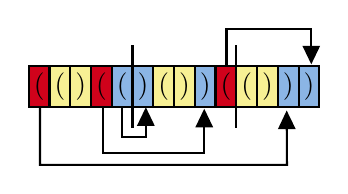
\begin{tikzpicture}[x=0.75pt,y=0.75pt,yscale=-1,xscale=1]
	\draw  [fill={rgb, 255:red, 208; green, 2; blue, 27 }  ,fill opacity=1 ] (160,170) -- (170,170) -- (170,190) -- (160,190) -- cycle;
	\draw  [fill={rgb, 255:red, 247; green, 240; blue, 148 }  ,fill opacity=1 ] (170,170) -- (180,170) -- (180,190) -- (170,190) -- cycle;
	\draw  [fill={rgb, 255:red, 247; green, 240; blue, 148 }  ,fill opacity=1 ] (180,170) -- (190,170) -- (190,190) -- (180,190) -- cycle;
	\draw  [fill={rgb, 255:red, 208; green, 2; blue, 27 }  ,fill opacity=1 ] (190,170) -- (200,170) -- (200,190) -- (190,190) -- cycle;
	\draw  [fill={rgb, 255:red, 139; green, 181; blue, 229 }  ,fill opacity=1 ] (200,170) -- (210,170) -- (210,190) -- (200,190) -- cycle;
	\draw  [fill={rgb, 255:red, 139; green, 181; blue, 229 }  ,fill opacity=1 ] (210,170) -- (220,170) -- (220,190) -- (210,190) -- cycle;
	\draw  [fill={rgb, 255:red, 247; green, 240; blue, 148 }  ,fill opacity=1 ] (220,170) -- (230,170) -- (230,190) -- (220,190) -- cycle;
	\draw  [fill={rgb, 255:red, 247; green, 240; blue, 148 }  ,fill opacity=1 ] (230,170) -- (240,170) -- (240,190) -- (230,190) -- cycle;
	\draw  [fill={rgb, 255:red, 139; green, 181; blue, 229 }  ,fill opacity=1 ] (240,170) -- (250,170) -- (250,190) -- (240,190) -- cycle;
	\draw  [fill={rgb, 255:red, 208; green, 2; blue, 27 }  ,fill opacity=1 ] (250,170) -- (260,170) -- (260,190) -- (250,190) -- cycle;
	\draw  [fill={rgb, 255:red, 247; green, 240; blue, 148 }  ,fill opacity=1 ] (260,170) -- (270,170) -- (270,190) -- (260,190) -- cycle;
	\draw  [fill={rgb, 255:red, 247; green, 240; blue, 148 }  ,fill opacity=1 ] (270,170) -- (280,170) -- (280,190) -- (270,190) -- cycle;
	\draw  [fill={rgb, 255:red, 139; green, 181; blue, 229 }  ,fill opacity=1 ] (280,170) -- (290,170) -- (290,190) -- (280,190) -- cycle;
	\draw  [fill={rgb, 255:red, 139; green, 181; blue, 229 }  ,fill opacity=1 ] (290,170) -- (300,170) -- (300,190) -- (290,190) -- cycle;
	\draw    (210,160) -- (210,200);
	\draw    (260,160) -- (260,200);
	\draw    (205.14,190.29) -- (205.14,204.36) -- (216.43,204.36) -- (216.43,192.93);
	\draw [shift={(216.43,189.93)}, rotate = 90] [fill={rgb, 255:red, 0; green, 0; blue, 0 }  ][line width=0.08]  [draw opacity=0] (8.93,-4.29) -- (0,0) -- (8.93,4.29) -- cycle;
	\draw    (195.57,189.79) -- (195.57,212.07) -- (244.57,212.07) -- (244.57,193.64);
	\draw [shift={(244.57,190.64)}, rotate = 90] [fill={rgb, 255:red, 0; green, 0; blue, 0 }  ][line width=0.08]  [draw opacity=0] (8.93,-4.29) -- (0,0) -- (8.93,4.29) -- cycle;
	\draw    (165.43,190.21) -- (165.43,217.64) -- (284.43,217.64) -- (284.3,194.5);
	\draw [shift={(284.29,191.5)}, rotate = 89.69] [fill={rgb, 255:red, 0; green, 0; blue, 0 }  ][line width=0.08]  [draw opacity=0] (8.93,-4.29) -- (0,0) -- (8.93,4.29) -- cycle;
	\draw    (255.29,170.21) -- (255.29,152.07) -- (296.14,152.07) -- (296.14,166.21);
	\draw [shift={(296.14,169.21)}, rotate = 270] [fill={rgb, 255:red, 0; green, 0; blue, 0 }  ][line width=0.08]  [draw opacity=0] (8.93,-4.29) -- (0,0) -- (8.93,4.29) -- cycle;

	\draw (161,172) node [anchor=north west][inner sep=0.75pt]   [align=left] {(};
	\draw (171,172) node [anchor=north west][inner sep=0.75pt]   [align=left] {(};
	\draw (181,172) node [anchor=north west][inner sep=0.75pt]   [align=left] {)};
	\draw (211,172) node [anchor=north west][inner sep=0.75pt]   [align=left] {)};
	\draw (201,172) node [anchor=north west][inner sep=0.75pt]   [align=left] {(};
	\draw (191,172) node [anchor=north west][inner sep=0.75pt]   [align=left] {(};
	\draw (271,172) node [anchor=north west][inner sep=0.75pt]   [align=left] {)};
	\draw (261,172) node [anchor=north west][inner sep=0.75pt]   [align=left] {(};
	\draw (251,172) node [anchor=north west][inner sep=0.75pt]   [align=left] {(};
	\draw (241,172) node [anchor=north west][inner sep=0.75pt]   [align=left] {)};
	\draw (231,172) node [anchor=north west][inner sep=0.75pt]   [align=left] {)};
	\draw (221,172) node [anchor=north west][inner sep=0.75pt]   [align=left] {(};
	\draw (291,172) node [anchor=north west][inner sep=0.75pt]   [align=left] {)};
	\draw (281,172) node [anchor=north west][inner sep=0.75pt]   [align=left] {)};
\end{tikzpicture}

	\caption{Divisione in blocchi di una parola di Dyck.}
	\label{fig:paren_blocks}
\end{figure}

\begin{lemma}[delle incrociate]\label{lem:dyckincro}
	In una parola di Dyck $w$, sia $p$ la posizione di una parentesi aperta. Allora
	\begin{equation*}
		\nexists q\mid p<q<\dyfindclosed(p) \quad\land\quad \dyfindclosed(q)>\dyfindclosed(p)
	\end{equation*}
\end{lemma}
\begin{proof}
	Se $p<q<\dyfindclosed(p)$ allora $E_w(q)>E_w(p)$. Poiché la funzione di eccesso non può scendere sotto il valore $E_w(q)$ senza raggiungere $\dyfindclosed(q)$, è impossibile che valga $\dyfindclosed(q)>\dyfindclosed(p)$.
\end{proof}

\noindent La struttura si compone di diverse componenti:
\begin{itemize}
	\item la parola $w$ memorizzata come sequenza di bit (un valore booleano per le parentesi aperte e l'altro per le chiuse).
	\item un vettore $E$ di $k$ elementi, contenente per ogni blocco il valore della funzione di eccesso nella sua prima posizione;
	\item un vettore $M$ che contiene, per ogni pioniera o relativa chiusa, l'indice della sua corrispondente;
	\item un vettore $O$ di $k$ elementi, contenente per ogni blocco l'ultima posizione prima di esso in cui la funzione di eccesso è minore del minimo in tale blocco;
	\item un vettore $\bar p$ di bit che identifica a $1$ le pioniere, a cui è associata una struttura succinta di rango e selezione;
\end{itemize}

\subsubsection{Implementazione dell'interfaccia}
\newcommand{\dyfindopenb}{\mathbf{find\_open}}
\newcommand{\dyfindclosedb}{\mathbf{find\_closed}}
\newcommand{\dyencloseb}{\mathbf{enclose}}
Per semplicità ci riferiremo con abuso di notazione ai simboli e alle rispettive posizioni intercambiabilmente.

\paragraph{$\dyfindclosedb$} È data la posizione $p$ di un'aperta. Sia $B=\floor{p/k}$ il blocco a cui $p$ appartiene.
L'algoritmo si compone dei seguenti passi:
\begin{enumerate}
	\item \label{en:dyfc:1} a partire da $E[B]$, ricavare l'eccesso $E_w(p)$ calcolando e salvando quello di ogni simbolo del blocco fino a $p$;
	\item calcolando gli eccessi delle posizioni successive a $p$ nel blocco, determinare se $p$ è vicina.
	      È così se e solo se esiste una posizione $r\neq p$ tale che $E_w(r)=E_w(p)$. Se si trova un tale $r$, restituire $r$; altrimenti $p$ è lontana;
	\item se $p$ è lontana allora si chiude in un blocco $B'\neq B$.
	      Se $\bar p[p]=1$ allora $p$ è una pioniera, precisamente la $(\rank_{\bar p}(p)+1)$-esima, quindi la chiusa corrispondente si trova in $M[\rank_{\bar p}(p)+1]$ e va restituito tale valore;
	\item se $\bar p_p=0$ allora $p$ non è una pioniera.
	      La pioniera precedente a $p$, ovvero la $(\rank_{\bar p}(p))$-esima, è la pioniera di riferimento di $p$, ossia è la pioniera in posizione $q=\select_{\bar p}(\rank_{\bar p}(p)-1)$ che si chiude nel blocco $B'$.
	      Se così non fosse si contraddirebbe il lemma \ref{lem:dyckincro} delle incrociate. Per lo stesso motivo la pioniera in posizione $q$ è aperta.
	      A partire dalla corrispondente chiusa $q'$ di $q$, in posizione $M[q]$, cercare verso sinistra a partire dalla posizione $q'$ la prima che ha eccesso $E_w(p)$.
	      L'eccesso di $q'$ è lo stesso di $q$, calcolato al passo \ref{en:dyfc:1}.
\end{enumerate}

\paragraph{$\dyfindopenb$} È data la posizione $p$ di una chiusa. Sia $B$ il blocco a cui $p$ appartiene.
L'algoritmo si compone dei seguenti passi:
\begin{enumerate}
	\item a partire da $E[B]$, ricavare l'eccesso $E_w(p)$ calcolando e salvando quello di ogni simbolo del blocco fino a $p$;
	\item se esistono posizioni tra quelle già analizzate con eccesso uguale a $E_w(p)$, restituire l'ultima: $p$ è vicina;
	\item dato che $p$ è lontana, se $\bar p[p]=1$ allora la parentesi in $p$ è una pioniera, precisamente la $(\rank_{\bar p}(p)+1)$-esima, quindi la chiusa corrispondente si trova in $M[\rank_{\bar p}(p)+1]$ e va restituito tale valore;
	\item se $\bar p_p=0$ allora $p$ non è una pioniera.
	      La pioniera successiva a $p$, è la $(\rank_{\bar p}(p)+1)$-esima, in posizione $q=\select_{\bar p}(\rank_{\bar p}(p))$.
	      Calcolare l'eccesso di $q$ procedendo verso destra a partire da $p$.
	      A partire dalla corrispondente aperta $q'$ di $q$, in posizione $M[q]$ e che ha lo stesso eccesso di $q$, cercare verso destra a partire dalla posizione $q'$ la prima che ha eccesso $E_w(p)$ e restituire il valore.
\end{enumerate}

\paragraph{$\dyencloseb$} È data una posizione $x$ in input.
Se $x$ è la posizione di un'aperta, sia $p:=x$ e $p':=\dyfindclosed_w(x)$, altrimenti sia $p=\dyfindopen_w(x)$ e $p'=x$.
Sia $B$ il blocco a cui $p$ appartiene.
L'algoritmo si compone dei seguenti passi:
\begin{enumerate}
	\item a partire da $E[B]$, ricavare l'eccesso $E_w(p)$, facendo in modo di mantenere in memoria l'ultima posizione $r$, se ne esiste una, per cui $E_w(r)=E_w(p)-1$;
	\item se $r$ esiste, restituire $r$;
	\item \label{en:dyen:3} sia $B'$ il blocco a cui appartiene $p'$ (si noti che non necessariamente $B'\neq B$).
	      Se esiste in tale blocco una posizione $r>p'$ tale che $E_w(r)=E_w(p')-1=E_w(p)-1$, restituire $\dyfindopen(r)$;
	\item si ha che $p$ ha il minimo eccesso in $B$.
	      Infatti, nelle posizioni minori di $p$ non è stato trovato l'eccesso $E_w(p)-1$, mentre per le posizioni maggiori vale uno dei seguenti casi:
	      \begin{itemize}
		      \item se $B'\neq B$, allora l'eccesso delle posizioni tra $p$ e $p'$ è almeno $E_w(p)$ in quanto ogni parentesi è avvolta da $p$ e $p'$;
		      \item se $B'=B$, allora per le posizioni successive a $p'$ si è visto al passo \ref{en:dyen:3} che non esiste posizione con eccesso uguale a $E_w(p)-1$.
	      \end{itemize}
	      restituire quindi $O[B]$.
\end{enumerate}

\begin{theorem}
	In una parola di Dyck $w$ divisa in $k\geq 2$ blocchi $B_1,\dots,B_k$, esistono $\card{\dypion(w)}\leq 2k-3$ pioniere.
\end{theorem}
% TODO: spostare in appendice?
\begin{proof}
	Per induzione su $k$:
	\begin{itemize}
		\item se $k=2$, si verifica uno e uno solo dei seguenti casi:
		      \begin{itemize}
			      \item nel primo blocco ogni parentesi è vicina, quindi il numero di pioniere è $0$. Quindi $\card{\dypion(w)}=0\leq 2k-3=1$;
			      \item esiste una sola pioniera in quanto ogni lontana in $B_1$ si chiude in $B_2$. Quindi $\card{\dypion(w)}=1\leq 2k-3=1$.
		      \end{itemize}
		\item per ipotesi induttiva, $\card{\dypion(w')}\leq 2k'-3~\forall k'<k,w'$. Si verifica uno e uno solo dei seguenti casi:
		      \begin{enumerate}
			      \item \label{en:dythm:1} se $w$ è debolmente bilanciata, esiste una posizione $p$ nel blocco $B_i$ entro cui tutte le pioniere aperte precedentemente si chiudono.
			            In questo caso, si considerino le parole $w':=w_1\cdots w_p$ e $w'':=w_{p+1}\cdots w_l$, che ereditano i blocchi da $w$ ottenendo $k'$ e $k''$ blocchi ($B_i$ è diviso tra le due ma presente in entrambe, così che $k=k'+k''-1$).
			            Poiché le pioniere di $w$ sono preservate, vale $\card{\dypion(w)}=\card{\dypion(w')}+\card{\dypion(w'')}$.
			            Poiché $w'$, $k'$, $w''$ e $k''$ sono tali da poter applicare l'ipotesi induttiva, vale
			            \begin{align*}
				            \card{\dypion(w)} & = \card{\dypion(w')}+\card{\dypion(w'')} \\
				                              & \leq (2k'-3)+(2k''-3)                    \\
				                              & = 2(k'+k''-3)                            \\
				                              & = 2(k-2) = 2k-4
			            \end{align*}
			      \item Se $w$ è fortemente bilanciata, allora esiste una pioniera che si apre nel primo blocco e si chiude nell'ultimo. Infatti, se così non fosse, sia $p$ la pioniera del primo blocco che si chiude nel blocco massimale (più lontano) $B_k$, con $k'<k$. Per il lemma \ref{lem:dyckincro} delle incrociate, le parentesi incluse tra $p$ e la sua chiusa $p'$ non possono chiudersi dopo $p'$. Inoltre la coppia $(p,p')$ non può essere racchiusa da un'altra coppia, altrimenti $p$ non sarebbe la pioniera che si chiude nel blocco massimale. Quindi l'eccesso in $p'$ è $0$, il che è assurdo.

			            Sia $p$ la prima pioniera di $w$. Si possono rimuovere coppie di parentesi che precedono $p$ o seguono la sua chiusa in quanto sono vicine e non contribuiscono al numero di pioniere. Si può inoltre rimuovere la parentesi $p$ e la relativa chiusa ottenendo una parola risultante $w'$ ancora bilanciata. Per $w'$ vale uno e uno solo dei seguenti casi:
			            \begin{itemize}
				            \item se si rimuove un intero blocco, ossia $k'<k$, si ha rimosso una pioniera. Per ipotesi induttiva $\dypion(w)=\dypion(w')+1\leq 2k'-3+1\leq 2k-4\leq 2k-3$;
				            \item se $w'$ è debolmente bilanciata, si ha rimosso una pioniera e si ricade nel caso \ref{en:dythm:1}. Quindi $\dypion(w)=\dypion(w')+1\leq 2k-4+1\leq 2k-3$;
				            \item se $w'$ è ancora fortemente bilanciata, selezionare una nuova pioniera $p'$ e ripetere il procedimento di rimozione appena descritto. Il numero di pioniere non cambia tra $w$ e $w'$.
			            \end{itemize}
		      \end{enumerate}
	\end{itemize}
\end{proof}

Lo spazio occupato in bit da queste strutture è:
\begin{equation*}
	\begin{aligned}
		 & w & n             \\
		 & E & k l           \\
		 & M & \leq 2(2k-3)l \\
		 & O & kl            \\
		 & p & n + o(n)
	\end{aligned}
\end{equation*}
Se si sceglie $l=\log_2 n$, si fa uso di un totale di al più $D_n=(6k-6)\log_2 n+2n+o(n)=8n+o(n)$ bit (ricordando che $k=\ceil{\frac nl}=\ceil{\frac{n}{\log_2 n}}<\frac{n}{\log_2 n}+1$).
Per confrontare questa grandezza con l'information theoretical lower bound consideriamo due insiemi isomorfi alle parentesi ben bilanciate: le foreste ordinate e gli alberi binari.


\subsection{Information theoretical lower bound}

\subsubsection{Parole di Dyck e foreste ordinate}
$F_n$, con $n\in\N$, è l'insieme delle foreste ordinate con $n$ nodi.
% TODO: essere più formali?
\begin{defin}
	Induttivamente:
	\begin{itemize}
		\item la foresta vuota $\seq{}$ appartiene a $F_0$;
		\item siano $f\in F_n$ e $g\in F_m$. Sia $\tree(f)$ l'albero ottenuto unendo sotto un'unica radice gli alberi di $f$. Allora $\seq{\tree(f),g}\in F_{n+m+1}$.
	\end{itemize}
\end{defin}

\begin{figure}[ht]
	\centering
	\begin{tikzpicture}[scale=0.8]
	\node[int] (T0) {} child { node[leaf] {}};

	\node[int,right=1.5cm of T0] (T1) {}
	child {node[leaf] {} }
	child {node[leaf] {} };

	\node[int,right=2.5cm of T1] (T1) {}
	child {node[int] {}
			child {node[leaf] {}}
		}
	child {node[leaf] {} }
	child {node[int] {}
			child {node[leaf] {}}
			child {node[leaf] {}}
		};
\end{tikzpicture}

	\caption{Foresta ordinata.}
	\label{fig:ordered_forest}
\end{figure}

Si consideri la funzione $\varphi:D_n\to F_n$, definita induttivamente come segue:
\begin{itemize}
	\item $\varphi(\emptyword)=\seq{}$;
	      % TODO: questa notazione è tecnicamente sbagliata in quanto ogni foresta sarebbe una coppia albero-foresta. Pensare a una notazione migliore
	\item $\varphi(~(w_1)w_2~)=\seq{\tree(\varphi(w_1)),\varphi(w_2)}$.
\end{itemize}

Come si può facilmente verificare la funzione descritta è biiettiva, in quanto una foresta ordinata appartiene a una e una sola delle forme delle immagini di $\varphi$.


\subsubsection{Foreste ordinate e alberi binari}
Si consideri la funzione $B:F_n\to B_n$ (dove $B_n$ è l'insieme degli alberi binari con $n$ nodi interni), definita induttivamente come segue:
% TODO: anche qui si potrebbe essere più formali. Per rivedere queste definizioni andrebbero riviste quelle di albero binario al relativo paragrafo
\begin{itemize}
	\item $B(\seq{})$ è l'albero costituito dalla sola radice;
	\item $B(\seq{\tree(f)},g)$ è l'albero binario costituito da una radice che ha per figlio sinistro $B(f)$ e destro $B(g)$.
\end{itemize}

\begin{figure}[ht]
	\centering
	% TODO: bruttissima, migliorare
	\begin{tikzpicture}[recurse/.style={rectangle,draw},scale=0.8]
	\node (T0) {$B\left(\left\langle\tikz\node[int,scale=0.6] {};, \raisebox{-2mm}{\tikz[scale=0.3,every node/.style={scale=0.6}] \node[int] {} child {node[leaf] {}};}\,\right\rangle\right)\,=$ };

	\node (T1) [above right=3mm and 13mm of T0,int] {}
	child[sibling distance=18mm] {node[recurse] {$B(\seq{})$} }
	child[sibling distance=18mm] {node[recurse] {$B\left(\left\langle\,\raisebox{-2mm}{\tikz[scale=0.3,every node/.style={scale=0.6}] \node[int] {} child {node[leaf] {}};}\,\right\rangle\right)$} };
	\node[right=31mm of T0] (u1) {$=$};

	\node (T2) [above right=3 mm and 29mm of T1,int] {}
	child {node[leaf] {} }
	child {node[int] {}
			child {node[recurse] {$B(\seq{\tikz\node[int,scale=0.6] {};})$}}
			child {node[recurse] {$B(\seq{})$}}
		};
	\node[right=24mm of u1] (u2) {$=$};

	\node (T3) [above right=2mm and 32mm of T2,int] {}
	child {node[leaf] {} }
	child {node[int] {}
			child {node[int] {}
					child {node[recurse] {$B(\seq{})$} }
					child {node[recurse] {$B(\seq{})$} }
				}
			child {node[leaf] {} }
		};
	\node[right=27mm of u2] {$=$};

	\node (T4) [right=2.7cm of T3,int] {}
	child {node[leaf] {} }
	child {node[int] {}
			child {node[int] {}
					child {node[leaf] {} }
					child {node[leaf] {} }
				}
			child {node[leaf] {} }
		};
\end{tikzpicture}

	\caption{Esempio di calcolo dell'isomorfismo tra foreste ordinate e alberi binari.}
	\label{fig:iso_forest_bintree_example}
\end{figure}

Dal momento che i tre insiemi sono isomorfi, le loro cardinalità sono uguali. Come visto al \cref{thm:catalano}:
\begin{equation*}
	\card{D_n}=\card{F_n}=\card{B_n}=C_n \text,
\end{equation*}
da cui
\begin{equation*}
	Z_n=\log_2(C_n)=2n-O(\log n) \text{ bit}.
\end{equation*}
Ergo, la struttura vista per l'ADT delle parentesi ben bilanciate che ha un costo in spazio di $8n+o(n)=O(Z_n)$ bit è compatta.



\section{Tecniche di hashing}
Una funzione di hash $h:U\to n$ associa ogni elemento di un universo $U$ a un numero da $0$ a $n-1$, detto bucket.

Se $U$ è finito, il numero di funzioni di hash con $n$ bucket su universo $U$ è $n^{|U|}$.

L'analisi che segue si basa su alcune assunzioni, solo approssimabili nella pratica\footnote{
	In genere, se $\Sigma$ è un alfabeto e $U=\Sigma^{\leq l}$, una funzione di hash $h: U\to n$ viene memorizzata tramite valori casuali $w=\angle{l_i}_{i\in l}$ inclusi tra $0$ e $\card\Sigma-1$ e calcolata come $h(s)=\left(\sum_{i=0}^{l-1} s_i w_i\right) \mod n$. Tipicamente vengono imposti vincoli su $n$ (ad esempio che sia primo). È facile vedere che questa tecnica non rispetta le condizioni.
}:
\begin{itemize}
	\item $h$ è calcolabile in tempo costante rispetto a $\card U$;
	\item $h$ occupa spazio costante rispetto a $\card U$;
	\item fissati $U$ e $n$ è possibile estrarre uniformemente a caso una funzione di hash $h:U\to n$ (\flang{full randomness assumption}).
\end{itemize}


\subsection{Sequenze di peeling di un grafo}
Le sequenze di peeling di un grafo generalizzano la nozione di aciclicità agli ipergrafi e forniscono una tecnica applicabile al metodo MWHC.

\begin{defin}
	Sia $G=(V,E)$ un grafo non orientato. Una sequenza di peeling per $G$ è una sequenza di coppie $\tuple{e_i,x_i}\in E\times V$, con $x_i\in e_i$, in cui appaiono tutti i lati e tale per cui nessun vertice $x_i$ (detto cardine o \flang{hinge}) appare nei lati $e_1,\dots,e_{i-1}$.
\end{defin}

\begin{figure}[ht]
	\begin{center}
		% TODO: pessimo esempio, migliorare
		\begin{subfigure}[b]{0.45\textwidth}
			\begin{center}
				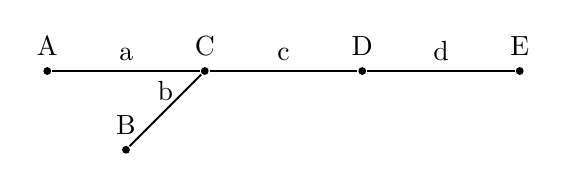
\begin{tikzpicture}
	\node [circle,fill,label=above:{A},inner sep=1pt](A) at (0,0) {};
	\node [circle,fill,label=above:{B},inner sep=1pt](B) at (1,-1) {};
	\node [circle,fill,label=above:{C},inner sep=1pt](C) at (2,0) {};
	\node [circle,fill,label=above:{D},inner sep=1pt](D) at (4,0) {};
	\node [circle,fill,label=above:{E},inner sep=1pt](E) at (6,0) {};

	\draw (A) -- (C) node [midway,above] {a};
	\draw (B) -- (C) node [midway,above] {b};
	\draw (C) -- (D) node [midway,above] {c};
	\draw (D) -- (E) node [midway,above] {d};
\end{tikzpicture}

			\end{center}
		\end{subfigure}
		\begin{subfigure}[b]{0.45\textwidth}
			\begin{center}
				\begin{align*}
					a & = \{(A, C), A\} \\
					b & = \{(B, C), B\} \\
					c & = \{(C, D), D\} \\
					d & = \{(D, E), E\}
				\end{align*}
			\end{center}
		\end{subfigure}
	\end{center}
	\caption{Un grafo e una sequenza di peeling valida.}%
	\label{fig:example_peeling}
\end{figure}

Il risultato fondamentale sulle sequenze di peeling lega la loro presenza a quella di cicli:
\begin{theorem}
	Un grafo ammette una sequenza di peeling se e solo se è aciclico.
\end{theorem}

\subsubsection{Sequenze di peeling di un ipergrafo}
Un $r$-ipergrafo uniforme $G=(V,E)$ è composto da un insieme $V$ di vertici e uno $E$ di iperlati, dove ogni iperlato è un insieme di $r$ vertici\footnote{Negli $r$-ipergrafi generici un iperlato ha al più $r$ vertici.} (i.e. $E\subseteq\binom{V}{r}$).

Le sequenze di peeling si definiscono sugli ipergrafi in modo del tutto analogo a quello per i grafi, come un insieme di coppie iperlato-cardine. Per definizione, un ipergrafo è aciclico se e solo se ammette una sequenza di peeling.



\subsection{La tecnica MWHC}
La tecnica MWHC\footnote{Da Majewski Wormald Havas Czech \cite{Majewski:96:MWHC}} ha lo scopo di memorizzare un dizionario statico (ossia immutabile).
Si consideri un insieme universo $U$ e un insieme $S\subset U$ di chiavi tale che $m:=\card S\ll\card U$. Si fissi inoltre una costante $r\in\N^+$.
Un dizionario $D$ ha in input un valore $x\in U$ e produce un output.
È data una funzione $f:S\to 2^r$ detta \emph{prescritta}: l'output di $D$ è $f(x)$ se $x\in S$, mentre può consistere in qualunque valore se $x\in U\setminus S$.

La tecnica MWHC permette di ricavare la prescritta in una data chiave senza la necessità di memorizzare alcuna chiave. Per fare ciò, vengono estratte casualmente due funzioni di hash $h_1,h_2:U\to n$.
Viene poi costruito un grafo non orientato $G=(V,E)$, dove $V=n$ e $E=\set{\set{h_1(x),h_2(x)}\mid x\in S}$ (quindi $\card E=m$).
Se si verifica una delle seguenti condizioni, l'estrazione di $h_1$ e $h_2$ viene ripetuta:
\begin{itemize}
	\item $\exists x,y\mid x\neq y\land \set{h_1(x),h_2(x)}=\set{h_1(y),h_2(y)}$;
	\item $\exists x\mid h_1(x)=h_2(x)$;
	\item $G$ contiene cicli.
\end{itemize}

Per poter calcolare i valori di $f$ senza doverli memorizzare, si costruisce un sistema di $m$ equazioni, una per ogni $x\in S$, del tipo
\begin{equation*}
	(w_{h_1(x)} + w_{h_2(x)}) \mod 2^r = f(x) \text,
\end{equation*}
dove $w_0,\dots,w_{n-1}$ sono variabili.

Poiché $G$ è aciclico esiste per esso una sequenza di peeling. Ordinando le equazioni come la sequenza (gli indici delle variabili corrispondenti agli elementi di ciascun arco) e risolvendo ciascuna equazione nel suo cardine, si può portare il sistema in una forma risolvibile trivialmente ("a gradini").

Memorizzate le soluzioni $w_i$ del sistema in un vettore $W$, si può calcolare $f(x)$ per un dato $x\in S$ con la formula
\begin{equation*}
	f(x) = (W[h_1(x)] + W[h_2(x)]) \mod 2^r
\end{equation*}

% TODO: necessario un esempio

Per quanto riguarda il dimensionamento di $n$, se $n\leq m$ allora il grafo è necessariamente ciclico ed è impossibile quindi determinare le funzioni di hash.
Per $n>m$, \cite{Majewski:96:MWHC} dimostra:
\begin{theorem}
	Se $n>2.09m$, la procedura di selezione di $h_1$ e $h_2$ termina in un numero atteso di $2$ tentativi.
\end{theorem}
Adattando la procedura all'utilizzo di un $3$-ipergrafo, il rapporto $\gamma$ tra $n$ e $m$ è minimo: $n>1.23m$.
Il costo in spazio di questa struttura è quello per salvare i valori di $n$ variabili di $r$ bit. Considerato il rapporto tra $n$ e $m$ regolato da $\gamma$, tale costo è di $\gamma rm$ bit. Poiché si sta memorizzando una funzione $f:m\to 2^r$ tra $(2^r)^m$ possibili, l'information theoretical lower bound è $rm$ e pertanto, essendo $\gamma$ costante, la struttura è compatta.

\subsubsection{MWHC compresso}
Il sistema della tecnica MWHC è indeterminato, con un numero di gradi di libertà di $n-m$. Ponendo le variabili libere a $0$, e mantenendo i valori non nulli solo per i cardini, si ottiene un vettore $W$ con al più $m$ valori non nulli.
È sufficiente quindi memorizzare $m$ valori per le variabili, sfruttando un array di $\gamma m$ bit, provvisto di struttura di rango, che indichi quali delle variabili totali sono non nulle.

Lo spazio occupato per questa struttura compressa è di $mr+\gamma m+o(m)=O(mr)$ bit, con un numero di bit per chiave di $r+\gamma$, contro i $r\gamma$ della versione non compressa.
Il suo utilizzo è quindi conveniente per $r>\frac{\gamma}{\gamma-1}$ ($r>5$ nel caso di $3$-ipergrafi).


\subsection{Hashing minimale perfetto}
Sia $U$ l'insieme universo e $S\subseteq U$, con $m:=\card S$. Una funzione di hash $H:U\to n$ si dice
\begin{description}
	\item[perfetta] per $S$ se $\forall s_1,s_2\in S:~H(s_1)=H(s_2)\impl s_1=s_2$ (se $H$ è "iniettiva" su $S$);
	\item[minimale] per $S$ se $n=\card S$.
\end{description}

Il problema di determinare una funzione di hashing minimale perfetto (MPHF, \flang{minimal perfect hashing function}) per un dato insieme $S$ viene risolto da una costruzione simile alla precedente. \cite{Majewski:96:MWHC}

Si vuole costruire una funzione $H:U\to m$ minimale e perfetta per $S$.
Questa volta si costruisce un sistema di equazioni del tipo
\begin{equation*}
	(w_{h_0(x)} + w_{h_1(x)} + w_{h_2(x)}) \mod 3 = k \text,
\end{equation*}
dove $k$ è l'indice della funzione di hash che determina il cardine della peeling sequence (i.e., $k=0$ se il cardine dell'iperlato $\set{h_0(x),h_1(x),h_2(x)}$ è $h_0(x)$, etc.).

Come per la tecnica MWHC, si risolve il sistema grazie alla sequenza di peeling e si salvano i valori delle variabili $w$ in un vettore $W$ di $m$ elementi, ciascuno di $2$ bit.
Si definisce poi la funzione $\bar H:U\to n$ calcolata come segue:
\begin{equation*}
	\bar H(x) = h_{(W[h_0(x)] + W[h_1(x)] + W[h_2(x)]) \mod 3}(x)
\end{equation*}
La funzione restituisce il valore del cardine dell'arco identificato da $x$, pertanto la funzione è perfetta (ossia, iniettiva su $S$).

La funzione non è, in generale, minimale, in quanto può restituire valori da $0$ a $n-1$.
Per renderla minimale è necessario "compattare" le immagini, nell'insieme $m$.
Per fare ciò, si consideri un vettore $p$ di rango composto da $n$ bit, il bit $i$ posto a $1$ se il vertice $i$ è cardine.
Ottenuta l'immagine $y=\bar H(x)$ di una stringa $x$, il rango di $y$ in tale vettore fornisce la suddetta compattazione, in quanto consiste nel numero di cardini minori di $i$.
Si ottiene quindi una funzione $H:U\to m$ minimale perfetta per $S$:
\begin{equation*}
	H(x) = \rank_p(\bar H(x))
	= \rank_p(h_{(W[h_0(x)] + W[h_1(x)] + W[h_2(x)]) \mod 3}(x))
\end{equation*}

Il costo spaziale dei due vettori $W$ e $p$ è di $2n+n=3n$ bit.
Per risparmiare $m$ bit, si consideri che dei quattro valori possibili per ciascun elemento di $W$ vengono usati solo tre valori.
Assegnando il valore $3$ agli elementi cardine a $0$, si lascia invariato l'output di $\bar H$ (per via del modulo $3$), ma si può effettuare l'operazione rango direttamente nel vettore $W$, poiché tutti e soli gli elementi diversi da $0$ sono cardini.
Il costo complessivo in bit è quindi di $2n$, ovvero di $2.46m$ se $\gamma=1.23$.
